\documentclass{article}
\usepackage{listings}
\usepackage{amsmath}
\usepackage{fullpage}
\usepackage{graphicx}
\usepackage{wrapfig}
\usepackage{longtable}
\usepackage[
	colorlinks=true,
	urlcolor=black,
	linkcolor=blue,
	citecolor = black,
	naturalnames=true,
	pdftitle={LIMES Web service},
	pdfsubject={Manual},
	pdfauthor={Klaus Lyko},
	pdfkeywords={LIMES, Link Discovery, Linked Data, Web service}
]{hyperref}
%%%%%%%%%%%%%%%%%%%%%%%%%%%%%%%%%%%%%%%%%%%%%%%%%%%%
\begin{document}

%\thispagestyle{empty}
% titlepage
\begin{titlepage}
	\begin{center}
		% Upper part of the page
		
\includegraphics[width=\textwidth]{images/limes_logo.pdf}
		\centering
		\huge Limes Web service User Manual
		\huge Version 0.1	
		\vfill
		% Bottom of the page
	%	\large \today
	\end{center}
\end{titlepage}
\tableofcontents
%%%%%%%%%%%%%%%%%%%%%%%%%%%%%%%%%%%%%%%%%%%%%%%
\newpage
\section{Introduction}
This document describes the LIMES Web service (LWS).\\
LWS was developed as a student project at the University of Leipzig in 2012 and is currently maintained by Klaus Lyko (University of Leipzig). 
Note, that LWS is still under development. Hence, all features remain in a beta status.

\subsection{Deployed version}
We deployed the current stable LWS version at: \url{http://139.18.2.164:8080/axis2/services/LimesServiceImpl} \\
The pre-built sample client could be downloaded at \url{139.18.2.164:8080/LimesWebService_Client.jar}.\\
If you notice some bugs feel free to post them at our GitHub repository: \url{https://github.com/KLyko/LimesWebService/}

\section{The Web service}
This section describes the features and basic architecture of the LWS.
\subsection{Features}
\begin{figure}[htbp]
	\centering
		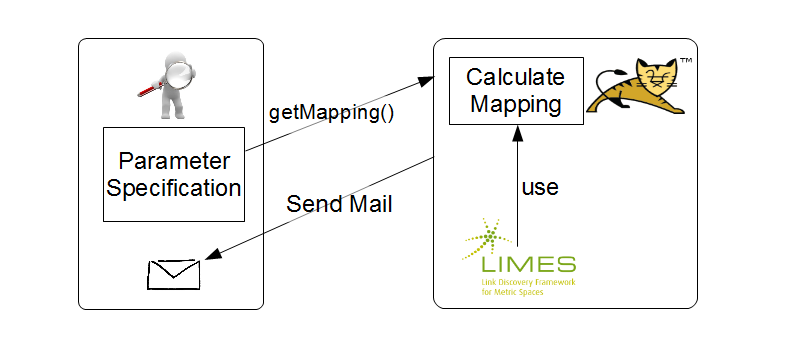
\includegraphics[width=7in]{images/limes_webservice_workflow_skizze_for_dummies.png}
	\caption{Basic workflow}
	\label{fig:limes_webservice_workflow_skizze_for_dummies}
\end{figure}
The main purpose of LWS is to provide a Web service to use the LIMES mapping mechanisms. Given a so-called Link Specification LWS provides the getMapping() method, which basically runs the LIMES framework with the given specifications. As the mapping process can last some time (above all querying large and/or slow endpoints) the method is designed asynchronous: Once, LIMES has finished calculation the Web service  will send an email with the results as attachment. Therefore, above all LWS expects that the user submitted an email address results will be send to.
Figure~\ref{fig:limes_webservice_workflow_skizze_for_dummies} depicts the basic work flow of LWS. First, a client has to start a session, submitting parameters such as an email address and the necessary LIMES Link Specification parameters. Finally, the client calls the getMapping() method to start the linking process. Once the server finishes calculation it sends the results as an email attachment. Figure~\ref{fig:workflow2} illustrates all these major methods and use cases of LWS.
\begin{figure}[h]
	\centering
		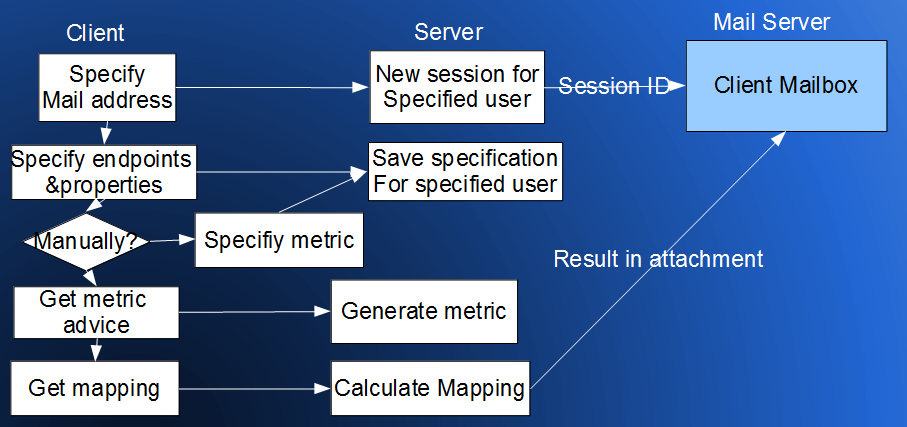
\includegraphics[width=7in]{images/workflow2.png}
	\caption{Workflow of LWS}
	\label{fig:workflow2}
\end{figure}

\subsection{Architecture}
We developed a basic Web service using the Apache Axis2\footnote{\url{http://axis.apache.org/axis2/java/core/}} framework. 

%%%%%%%%%%%%%%%%%%%%%
\newpage
\section{The Client}
A client working for LWS was built with JAVA and can be downloaded as a pre-built jar at \url{https://github.com/KLyko/LimesWebService/}. As the Web service is designed to work asynchronous all actions require to start a new session.\\
\begin{figure}[h]
	\centering
		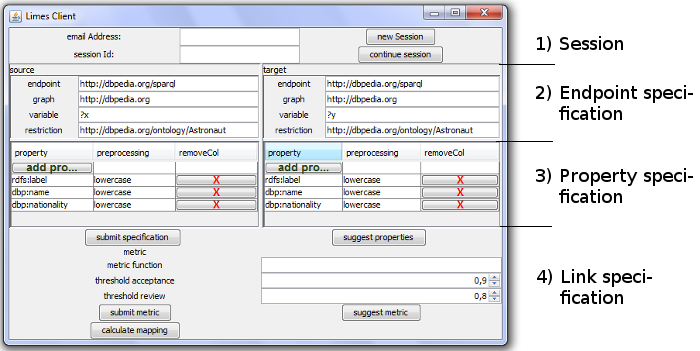
\includegraphics[width=7in]{images/Client_tasks.png}
	\caption{GUI of the client application. The basic steps are represented as horizontal layers. The basic work flow follows a top-down usage of the client.}
	\label{fig:client_tasks}
\end{figure}
As illustrated in figure \ref{fig:client_tasks} the basic steps are:
\begin{enumerate}
	\item Enter your email address and press \textit{create new session}. You will receive an email from the web service with the session id. This id is valid for 2 days. With it you can resume an older session.
	\item Specify both SPARQL endpoints.
	\item Specify the properties of both knowledge bases. 
	\item Specify a link specification using the LIMES specific link specification language. Either enter inter manually or use the unsupervised advise method.
	%\item Perform the mapping process using above settings by pressing \textit{calculate mapping}. Results will be send to your email address.
\end{enumerate}
Once you completed steps 1-2 you can submit the endpoint specification by clicking \textit{submit specification}. To submit a link specification click \textit{submit metric}. The server is now ready to perform the linking task. Start the (asynchronous) linking process by clicking \textit{start mapping}. The results will be send to your email address. This may take some time.
The following subsections will describe these discrete steps in more detail.

\subsection{Session start}
You can either start a new session or try to continue an older session. To start a new session enter your email address and click \textit{new Session}. The generated session id will be send to you by email.\\ You can continue old session withing 2 days by entering the session id and clicking \textit{continue session}. If old specification have been submitted, the client will load them.
\subsection{Endpoint specification}
On start-up the client is pre-configured with a example specification. As the endpoint layer suggests you have to enter the following parameters for each SPARQL endpoint:

\begin{enumerate}
	\item The URL of the SPARQL endpoint.
	\item The graph pattern (optional)
	\item The variable to reference the endpoint in the link specification. A variable name begins with a question mark. You may leave the default \texttt{?x} for the source and \texttt{?y} for the target endpoint untouched.
	\item Enter a class restriction. This is the URI of the \texttt{rdf:type} property.
\end{enumerate}

\subsection{Specification of the properties}
The next step is to specify which properties of the instances of each endpoint you want to use for the matching task. You can either use fully qualified URIs or abbreviated URIs utilizing well-known prefixes. Please refer to the appendix for a complete list of the available prefixes\footnote{A more convenient way to specify the properties is subject to future developments.}.\\Each property can be assigned to a specific preprocessing step. Please refer to the LIMES manual on details on available preprocessing functions., The most common are \texttt{lowercase} and \texttt{nolang}. Multiple preprocessing function can be concatenated using \texttt{->}, e.g. \texttt{lowercase->nolang}. With the \textit{add property} and the \textit{x} button you can create additional rows for properties, or remove them respectively.\\ \\
Once you specified both endpoints and the properties to use, you can submit the specification with the \textit{submit specification}  button.
%Note, the \textit{suggest properties} button has no function yet. Just ignore it for the time being.
\subsection{Link specification}
Once both endpoints are configured and you submitted the configuration using the \textit{submit specification}  button, the next step is to design the comparison pattern using the flexible LIMES link specification language. Both the metric expression and the global thresholds have to be set. There are to two ways to do that: 1. Manual enter the metric expression (field \textit{metric function} and set both thresholds. 2. Use the LIMES suggestion function.\\
\subsubsection{Manual configuration}
Enter the link specification (metric expression) using the defined variables and properties (either refer to them by there full URI or use the prefixes to enter abbreviated URIs). Either way for details on how to use the LIMES link specification language you may refer to the LIMES manual\footnote{\url{http://wiki.aksw.org/Projects/LIMES?show_comments=1}}.
\subsubsection{Use automatic link specification advise}
LIMES comes with a unsupervised learning mechanism to compute link specifications, called self-configuration. This feature of the LWS is implemented in a synchronous manner. To start the self-configuration for the specified knowledge bases, click the \textit{get metric advice} button. The computation of a link specification suggestion could take some time. So, you may have to wait several minutes for a response from the server. Once the suggestion is computed the proposed link specification will be written to the \textit{metric function} field.

\appendix
\section{List of known prefixes}
List of known prefixes of the client. Prefixes can be used to abbreviate URIs of properties.

\begin{longtable}{ c | p{8cm} }
  prefix & URI \\
  \hline                        
		abc & \url{http://www.metadata.net/harmony/ABCSchemaV5Commented.rdf#} \\
		ac & \url{http://umbel.org/umbel/ac/} \\
		acc & \url{http://purl.org/NET/acc#} \\
		acl & \url{http://www.w3.org/ns/auth/acl#} \\
		acm & \url{http://www.rkbexplorer.com/ontologies/acm#} \\
		act & \url{http://www.w3.org/2007/rif-builtin-action#} \\
		ad & \url{http://schemas.talis.com/2005/address/schema#} \\
		admin & \url{http://webns.net/mvcb/} \\
		af & \url{http://purl.org/ontology/af/} \\
		affy & \url{http://www.affymetrix.com/community/publications/affymetrix/tmsplice#} \\
		afn & \url{http://jena.hpl.hp.com/ARQ/function#} \\
		agent & \url{http://eulersharp.sourceforge.net/2003/03swap/agent#} \\
		agents & \url{http://eulersharp.sourceforge.net/2003/03swap/agent#} \\
		aifb & \url{http://www.aifb.kit.edu/id/} \\
		aiiso & \url{http://purl.org/vocab/aiiso/schema#} \\
		air & \url{http://dig.csail.mit.edu/TAMI/2007/amord/air#} \\
		airport & \url{http://www.daml.org/2001/10/html/airport-ont#} \\
		akt & \url{http://www.aktors.org/ontology/portal#} \\
		akts & \url{http://www.aktors.org/ontology/support#} \\
		am & \url{http://vocab.deri.ie/am#} \\
		anca & \url{http://www.semanticweb.org/ontologies/2010/6/Ontology1279614123500.owl#} \\
		ao & \url{http://purl.org/ontology/ao/core#} \\
		arch & \url{http://purl.org/archival/vocab/arch#} \\
		ass & \url{http://uptheasset.org/ontology#} \\
		atom & \url{http://www.w3.org/2005/Atom/} \\
		atomix & \url{http://buzzword.org.uk/rdf/atomix#} \\
		audio & \url{http://purl.org/media/audio#} \\
		awol & \url{http://bblfish.net/work/atom-owl/2006-06-06/#} \\
		bib & \url{http://zeitkunst.org/bibtex/0.1/bibtex.owl#} \\
		bibbaseontology & \url{http://data.bibbase.org/ontology/#} \\
		biblio & \url{http://purl.org/net/biblio#} \\
		bibo & \url{http://purl.org/ontology/bibo/} \\
		bibtex & \url{http://purl.oclc.org/NET/nknouf/ns/bibtex#} \\
		bill & \url{http://www.rdfabout.com/rdf/schema/usbill/} \\
		bio & \url{http://purl.org/vocab/bio/0.1/} \\
		bio2rdf & \url{http://bio2rdf.org/} \\
		biol & \url{http://purl.org/NET/biol/ns#} \\
		bioskos & \url{http://eulersharp.sourceforge.net/2003/03swap/bioSKOSSchemes#} \\
		book & \url{http://purl.org/NET/book/vocab#} \\
		botany & \url{http://purl.org/NET/biol/botany#} \\
		bsbm & \url{http://www4.wiwiss.fu-berlin.de/bizer/bsbm/v01/vocabulary/} \\
		c4n & \url{http://vocab.deri.ie/c4n#} \\
		c4o & \url{http://purl.org/spar/c4o/} \\
		cal & \url{http://www.w3.org/2002/12/cal/ical#} \\
		care & \url{http://eulersharp.sourceforge.net/2003/03swap/care#} \\
		cc & \url{http://creativecommons.org/ns#} \\
		ccard & \url{http://purl.org/commerce/creditcard#} \\
		cco & \url{http://purl.org/ontology/cco/core#} \\
		cert & \url{http://www.w3.org/ns/auth/cert#} \\
		cfp & \url{http://sw.deri.org/2005/08/conf/cfp.owl#} \\
		chord & \url{http://purl.org/ontology/chord/} \\
		cito & \url{http://purl.org/net/cito/} \\
		cld & \url{http://purl.org/cld/terms/} \\
		climb & \url{http://climb.dataincubator.org/vocabs/climb/} \\
		clineva & \url{http://www.agfa.com/w3c/2009/clinicalEvaluation#} \\
		clinproc & \url{http://www.agfa.com/w3c/2009/clinicalProcedure#} \\
		cmp & \url{http://www.ontologydesignpatterns.org/cp/owl/componency.owl#} \\
		cnt & \url{http://www.w3.org/2008/content#} \\
		co & \url{http://purl.org/ontology/co/core#} \\
		code & \url{http://telegraphis.net/ontology/measurement/code#} \\
		coin & \url{http://purl.org/court/def/2009/coin#} \\
		com & \url{http://purl.org/commerce#} \\
		commerce & \url{http://purl.org/commerce#} \\
		common & \url{http://www.w3.org/2007/uwa/context/common.owl#} \\
		compass & \url{http://purl.org/net/compass#} \\
		con & \url{http://www.w3.org/2000/10/swap/pim/contact#} \\
		conserv & \url{http://conserv.deri.ie/ontology#} \\
		contact & \url{http://www.w3.org/2000/10/swap/pim/contact#} \\
		content & \url{http://purl.org/rss/1.0/modules/content/} \\
		conv & \url{http://purl.org/twc/vocab/conversion/} \\
		conversion & \url{http://purl.org/twc/vocab/conversion/} \\
		copyright & \url{http://rhizomik.net/ontologies/2008/05/copyrightonto.owl#} \\
		coref & \url{http://www.rkbexplorer.com/ontologies/coref#} \\
		cos & \url{http://www.inria.fr/acacia/corese#} \\
		countries & \url{http://eulersharp.sourceforge.net/2003/03swap/countries#} \\
		courseware & \url{http://courseware.rkbexplorer.com/ontologies/courseware#} \\
		cpm & \url{http://catalogus-professorum.org/cpm/} \\
		crm & \url{http://purl.org/NET/cidoc-crm/core#} \\
		crypto & \url{http://www.w3.org/2000/10/swap/crypto#} \\
		cs & \url{http://purl.org/vocab/changeset/schema#} \\
		ct & \url{http://data.linkedct.org/resource/linkedct/} \\
		ctag & \url{http://commontag.org/ns#} \\
		custom & \url{http://www.openrdf.org/config/sail/custom#} \\
		cv & \url{http://rdfs.org/resume-rdf/} \\
		cyc & \url{http://sw.opencyc.org/concept/} \\
		cycann & \url{http://sw.cyc.com/CycAnnotations_v1#} \\
		d2rq & \url{http://www.wiwiss.fu-berlin.de/suhl/bizer/D2RQ/0.1#} \\
		dady & \url{http://purl.org/NET/dady#} \\
		daia & \url{http://purl.org/ontology/daia/} \\
		dailymed & \url{http://www4.wiwiss.fu-berlin.de/dailymed/resource/dailymed/} \\
		daml & \url{http://www.daml.org/2001/03/daml+oil#} \\
		days & \url{http://ontologi.es/days#} \\
		dayta & \url{http://dayta.me/resource#} \\
		dblp & \url{http://www4.wiwiss.fu-berlin.de/dblp/terms.rdf#} \\
		dbo & \url{http://dbpedia.org/ontology/} \\
		dbp & \url{http://dbpedia.org/property/} \\
		dbpedia & \url{http://dbpedia.org/resource/} \\
		dbpediaowl & \url{http://dbpedia.org/ontology/} \\
		dbpp & \url{http://dbpedia.org/property/} \\
		dbpprop & \url{http://dbpedia.org/property/} \\
		dbr & \url{http://dbpedia.org/resource/} \\
		dc & \url{http://purl.org/dc/terms/} \\
		dc11 & \url{http://purl.org/dc/elements/1.1/} \\
		dcam & \url{http://purl.org/dc/dcam/} \\
		dcat & \url{http://vocab.deri.ie/dcat#} \\
		dcmit & \url{http://purl.org/dc/dcmitype/} \\
		dcmitype & \url{http://purl.org/dc/dcmitype/} \\
		dcn & \url{http://www.w3.org/2007/uwa/context/deliverycontext.owl#} \\
		dcq & \url{http://purl.org/dc/terms/} \\
		dct & \url{http://purl.org/dc/terms/} \\
		dcterm & \url{http://purl.org/dc/terms/} \\
		dcterms & \url{http://purl.org/dc/terms/} \\
		dctype & \url{http://purl.org/dc/dcmitype/} \\
		ddc & \url{http://purl.org/NET/decimalised#} \\
		ddl & \url{http://purl.org/vocab/riro/ddl#} \\
		derecho & \url{http://purl.org/derecho#} \\
		dgfoaf & \url{http://west.uni-koblenz.de/ontologies/2010/07/dgfoaf.owl#} \\
		dir & \url{http://schemas.talis.com/2005/dir/schema#} \\
		disease & \url{http://www.agfa.com/w3c/2009/humanDisorder#} \\
		diseasome & \url{http://www4.wiwiss.fu-berlin.de/diseasome/resource/diseasome/} \\
		dnr & \url{http://www.dotnetrdf.org/configuration#} \\
		doac & \url{http://ramonantonio.net/doac/0.1/#} \\
		doap & \url{http://usefulinc.com/ns/doap#} \\
		doc & \url{http://www.w3.org/2000/10/swap/pim/doc#} \\
		doclist & \url{http://www.junkwork.net/xml/DocumentList#} \\
		drug & \url{http://www.agfa.com/w3c/2009/drugTherapy#} \\
		drugbank & \url{http://www4.wiwiss.fu-berlin.de/drugbank/resource/drugbank/} \\
		drugbankvocab & \url{http://www4.wiwiss.fu-berlin.de/drugbank/vocab/resource/class/} \\
		dul & \url{http://www.loa-cnr.it/ontologies/DUL.owl#} \\
		dummy & \url{http://hello.com/} \\
		dv & \url{http://rdf.data-vocabulary.org/#} \\
		ean & \url{http://openean.kaufkauf.net/id/} \\
		earl & \url{http://www.w3.org/ns/earl#} \\
		ecs & \url{http://rdf.ecs.soton.ac.uk/ontology/ecs#} \\
		elog & \url{http://eulersharp.sourceforge.net/2003/03swap/log-rules#} \\
		enc & \url{http://www.w3.org/2001/04/xmlenc#} \\
		environ & \url{http://eulersharp.sourceforge.net/2003/03swap/environment#} \\
		es & \url{http://eulersharp.sourceforge.net/2003/03swap/log-rules#} \\
		esd & \url{http://def.esd.org.uk/} \\
		eu & \url{http://eulersharp.sourceforge.net/2003/03swap/log-rules#} \\
		event & \url{http://purl.org/NET/c4dm/event.owl#} \\
		events & \url{http://eulersharp.sourceforge.net/2003/03swap/event#} \\
		evopat & \url{http://ns.aksw.org/Evolution/} \\
		evset & \url{http://dsnotify.org/vocab/eventset/0.1/} \\
		ex & \url{http://example.org/} \\
		exif & \url{http://www.w3.org/2003/12/exif/ns#} \\
		ezcontext & \url{http://ontologies.ezweb.morfeo-project.org/ezcontext/ns#} \\
		eztag & \url{http://ontologies.ezweb.morfeo-project.org/eztag/ns#} \\
		factbook & \url{http://www4.wiwiss.fu-berlin.de/factbook/ns#} \\
		fb & \url{http://rdf.freebase.com/ns/} \\
		fec & \url{http://www.rdfabout.com/rdf/schema/usfec/} \\
		fed & \url{http://www.openrdf.org/config/sail/federation#} \\
		film & \url{http://data.linkedmdb.org/resource/film/} \\
		fn & \url{http://www.w3.org/2005/xpath-functions#} \\
		foaf & \url{http://xmlns.com/foaf/0.1/} \\
		formats & \url{http://www.w3.org/ns/formats/} \\
		frbr & \url{http://purl.org/vocab/frbr/core#} \\
		frbre & \url{http://purl.org/vocab/frbr/extended#} \\
		freebase & \url{http://rdf.freebase.com/ns/} \\
		fresnel & \url{http://www.w3.org/2004/09/fresnel#} \\
		game & \url{http://data.totl.net/game/} \\
		gen & \url{http://www.w3.org/2006/gen/ont#} \\
		genab & \url{http://eulersharp.sourceforge.net/2003/03swap/genomeAbnormality#} \\
		geo & \url{http://www.w3.org/2003/01/geo/wgs84_pos#} \\
		geodata & \url{http://sws.geonames.org/} \\
		geoes & \url{http://geo.linkeddata.es/page/ontology/} \\
		geographis & \url{http://telegraphis.net/ontology/geography/geography#} \\
		geonames & \url{http://www.geonames.org/ontology#} \\
		geospecies & \url{http://rdf.geospecies.org/ont/geospecies#} \\
		giving & \url{http://ontologi.es/giving#} \\
		gob & \url{http://purl.org/ontology/last-fm/} \\
		gold & \url{http://purl.org/linguistics/gold/} \\
		gpt & \url{http://purl.org/vocab/riro/gpt#} \\
		gr & \url{http://purl.org/goodrelations/v1#} \\
		grddl & \url{http://www.w3.org/2003/g/data-view#} \\
		gridworks & \url{http://purl.org/net/opmv/types/gridworks#} \\
		gv & \url{http://rdf.data-vocabulary.org/#} \\
		h5 & \url{http://buzzword.org.uk/rdf/h5#} \\
		hard & \url{http://www.w3.org/2007/uwa/context/hardware.owl#} \\
		hartigprov & \url{http://purl.org/net/provenance/ns#} \\
		hcterms & \url{http://purl.org/uF/hCard/terms/} \\
		healthcare & \url{http://www.agfa.com/w3c/2009/healthCare#} \\
		hemogram & \url{http://www.agfa.com/w3c/2009/hemogram#} \\
		hlisting & \url{http://sindice.com/hlisting/0.1/} \\
		hospital & \url{http://www.agfa.com/w3c/2009/hospital#} \\
		http & \url{http://www.w3.org/2006/http#} \\
		httph & \url{http://www.w3.org/2007/ont/httph#} \\
		human & \url{http://eulersharp.sourceforge.net/2003/03swap/human#} \\
		humanbody & \url{http://eulersharp.sourceforge.net/2003/03swap/humanBody#} \\
		ibis & \url{http://purl.org/ibis#} \\
		ical & \url{http://www.w3.org/2002/12/cal/ical#} \\
		imm & \url{http://schemas.microsoft.com/imm/} \\
		imreg & \url{http://www.w3.org/2004/02/image-regions#} \\
		infection & \url{http://www.agfa.com/w3c/2009/infectiousDisorder#} \\
		ir & \url{http://www.ontologydesignpatterns.org/cp/owl/informationrealization.owl#} \\
		ire & \url{http://www.ontologydesignpatterns.org/cpont/ire.owl#} \\
		irrl & \url{http://www.ontologydesignpatterns.org/cp/owl/informationobjectsandrepresentationlanguages.owl#} \\
		irw & \url{http://www.ontologydesignpatterns.org/ont/web/irw.owl#} \\
		is & \url{http://purl.org/ontology/is/core#} \\
		isi & \url{http://purl.org/ontology/is/inst/} \\
		isq & \url{http://purl.org/ontology/is/quality/} \\
		ist & \url{http://purl.org/ontology/is/types/} \\
		iswc & \url{http://annotation.semanticweb.org/2004/iswc#} \\
		java & \url{http://www.w3.org/2007/uwa/context/java.owl#} \\
		jdbc & \url{http://d2rq.org/terms/jdbc/} \\
		kwijibo & \url{http://kwijibo.talis.com/} \\
		label & \url{http://purl.org/net/vocab/2004/03/label#} \\
		lang & \url{http://ontologi.es/lang/core#} \\
		languages & \url{http://eulersharp.sourceforge.net/2003/03swap/languages#} \\
		lark1 & \url{http://users.utcluj.ro/~raluca/ontology/Ontology1279614123500.owl#} \\
		lastfm & \url{http://purl.org/ontology/last-fm/} \\
		ldap & \url{http://purl.org/net/ldap/} \\
		lfm & \url{http://purl.org/ontology/last-fm/} \\
		lfn & \url{http://www.dotnetrdf.org/leviathan#} \\
		lgd & \url{http://linkedgeodata.org/vocabulary#} \\
		lgdo & \url{http://linkedgeodata.org/ontology/} \\
		lgdp & \url{http://linkedgeodata.org/property/} \\
		lib & \url{http://schemas.talis.com/2005/library/schema#} \\
		lifecycle & \url{http://purl.org/vocab/lifecycle/schema#} \\
		like & \url{http://ontologi.es/like#} \\
		lingvoj & \url{http://www.lingvoj.org/ontology#} \\
		link & \url{http://www.w3.org/2006/link#} \\
		linkedct & \url{http://data.linkedct.org/resource/linkedct/} \\
		list & \url{http://www.w3.org/2000/10/swap/list#} \\
		loc & \url{http://www.w3.org/2007/uwa/context/location.owl#} \\
		lode & \url{http://linkedevents.org/ontology/} \\
		log & \url{http://www.w3.org/2000/10/swap/log#} \\
		lom & \url{http://ltsc.ieee.org/rdf/lomv1p0/lom#} \\
		lomvoc & \url{http://ltsc.ieee.org/rdf/lomv1p0/vocabulary#} \\
		lotico & \url{http://www.lotico.com/meetup/} \\
		loticoowl & \url{http://www.lotico.com/ontology/} \\
		lp & \url{http://launchpad.net/rdf/launchpad#} \\
		lt & \url{http://diplomski.nelakolundzija.org/LTontology.rdf#} \\
		lvont & \url{http://lexvo.org/ontology#} \\
		lx & \url{http://purl.org/NET/lx#} \\
		ma & \url{http://www.w3.org/ns/ma-ont#} \\
		malignneo & \url{http://www.agfa.com/w3c/2009/malignantNeoplasm#} \\
		math & \url{http://www.w3.org/2000/10/swap/math#} \\
		media & \url{http://purl.org/microformat/hmedia/} \\
		meetup & \url{http://www.lotico.com/meetup/} \\
		memo & \url{http://ontologies.smile.deri.ie/2009/02/27/memo#} \\
		meta & \url{http://www.openrdf.org/rdf/2009/metadata#} \\
		meteo & \url{http://purl.org/ns/meteo#} \\
		mf & \url{http://poshrdf.org/ns/mf#} \\
		mit & \url{http://purl.org/ontology/mo/mit#} \\
		mo & \url{http://purl.org/ontology/mo/} \\
		moat & \url{http://moat-project.org/ns#} \\
		money & \url{http://purl.org/net/rdf-money/} \\
		movie & \url{http://data.linkedmdb.org/resource/movie/} \\
		mu & \url{http://www.kanzaki.com/ns/music#} \\
		music & \url{http://musicontology.com/} \\
		musim & \url{http://purl.org/ontology/similarity/} \\
		myspace & \url{http://purl.org/ontology/myspace#} \\
		myspo & \url{http://purl.org/ontology/myspace#} \\
		mysql & \url{http://web-semantics.org/ns/mysql/} \\
		nao & \url{http://www.semanticdesktop.org/ontologies/2007/08/15/nao#} \\
		ncal & \url{http://www.semanticdesktop.org/ontologies/2007/04/02/ncal#} \\
		nco & \url{http://www.semanticdesktop.org/ontologies/2007/03/22/nco#} \\
		ne & \url{http://umbel.org/umbel/ne/} \\
		net & \url{http://www.w3.org/2007/uwa/context/network.owl#} \\
		nexif & \url{http://www.semanticdesktop.org/ontologies/2007/05/10/nexif#} \\
		nfo & \url{http://www.semanticdesktop.org/ontologies/2007/03/22/nfo#} \\
		nid3 & \url{http://www.semanticdesktop.org/ontologies/2007/05/10/nid3#} \\
		nie & \url{http://www.semanticdesktop.org/ontologies/2007/01/19/nie#} \\
		nmo & \url{http://www.semanticdesktop.org/ontologies/2007/03/22/nmo#} \\
		nndsr & \url{http://semanticdiet.com/schema/usda/nndsr/} \\
		nrl & \url{http://www.semanticdesktop.org/ontologies/2007/08/15/nrl#} \\
		nsa & \url{http://multimedialab.elis.ugent.be/organon/ontologies/ninsuna#} \\
		nt & \url{http://ns.inria.fr/nicetag/2010/09/09/voc#} \\
		oat & \url{http://openlinksw.com/schemas/oat/} \\
		oauth & \url{http://demiblog.org/vocab/oauth#} \\
		obj & \url{http://www.openrdf.org/rdf/2009/object#} \\
		oc & \url{http://opencoinage.org/rdf/} \\
		odp & \url{http://ontologydesignpatterns.org/} \\
		og & \url{http://opengraphprotocol.org/schema/} \\
		ok & \url{http://okkam.org/terms#} \\
		okkam & \url{http://models.okkam.org/ENS-core-vocabulary#} \\
		olo & \url{http://purl.org/ontology/olo/core#} \\
		omb & \url{http://purl.org/ontomedia/ext/common/being#} \\
		omc & \url{http://purl.org/ontomedia/ext/common/bestiary#} \\
		ome & \url{http://purl.org/ontomedia/core/expression#} \\
		omm & \url{http://purl.org/ontomedia/core/media#} \\
		omp & \url{http://purl.org/ontomedia/ext/common/profession#} \\
		omt & \url{http://purl.org/ontomedia/ext/common/trait#} \\
		oo & \url{http://purl.org/openorg/} \\
		openlinks & \url{http://www.openlinksw.com/schemas/virtrdf#} \\
		opensearch & \url{http://a9.com/-/spec/opensearch/1.1/} \\
		opm & \url{http://openprovenance.org/ontology#} \\
		opmv & \url{http://purl.org/net/opmv/ns#} \\
		opo & \url{http://online-presence.net/opo/ns#} \\
		opus & \url{http://lsdis.cs.uga.edu/projects/semdis/opus#} \\
		opwn & \url{http://www.ontologyportal.org/WordNet.owl#} \\
		ore & \url{http://www.openarchives.org/ore/terms/} \\
		org & \url{http://www.w3.org/ns/org#} \\
		organism & \url{http://eulersharp.sourceforge.net/2003/03swap/organism#} \\
		organiz & \url{http://eulersharp.sourceforge.net/2003/03swap/organization#} \\
		os & \url{http://www.w3.org/2000/10/swap/os#} \\
		osag & \url{http://www.ordnancesurvey.co.uk/ontology/AdministrativeGeography/v2.0/AdministrativeGeography.rdf#} \\
		osgb & \url{http://data.ordnancesurvey.co.uk/id/} \\
		osoc & \url{http://web-semantics.org/ns/opensocial#} \\
		ov & \url{http://open.vocab.org/terms/} \\
		owl & \url{http://www.w3.org/2002/07/owl#} \\
		owlim & \url{http://www.ontotext.com/trree/owlim#} \\
		p3p & \url{http://www.w3.org/2002/01/p3prdfv1#} \\
		pbo & \url{http://purl.org/ontology/pbo/core#} \\
		pdo & \url{http://ontologies.smile.deri.ie/pdo#} \\
		pgterms & \url{http://www.gutenberg.org/2009/pgterms/} \\
		phss & \url{http://ns.poundhill.com/phss/1.0/} \\
		pimo & \url{http://www.semanticdesktop.org/ontologies/2007/11/01/pimo#} \\
		ping & \url{http://purl.org/net/pingback/} \\
		play & \url{http://uriplay.org/spec/ontology/#} \\
		plink & \url{http://buzzword.org.uk/rdf/personal-link-types#} \\
		pmlj & \url{http://inference-web.org/2.0/pml-justification.owl#} \\
		pmlp & \url{http://inference-web.org/2.0/pml-provenance.owl#} \\
		pmlr & \url{http://inference-web.org/2.0/pml-relation.owl#} \\
		pmlt & \url{http://inference-web.org/2.0/pml-trust.owl#} \\
		pmt & \url{http://tipsy.googlecode.com/svn/trunk/vocab/pmt#} \\
		po & \url{http://purl.org/ontology/po/} \\
		pobo & \url{http://purl.obolibrary.org/obo/} \\
		politico & \url{http://www.rdfabout.com/rdf/schema/politico/} \\
		posh & \url{http://poshrdf.org/ns/posh/} \\
		postcode & \url{http://data.ordnancesurvey.co.uk/id/postcodeunit/} \\
		powder & \url{http://www.w3.org/2007/05/powder#} \\
		pr & \url{http://ontologi.es/profiling#} \\
		prj & \url{http://purl.org/stuff/project/} \\
		product & \url{http://purl.org/commerce/product#} \\
		profiling & \url{http://ontologi.es/profiling#} \\
		prot & \url{http://www.proteinontology.info/po.owl#} \\
		protege & \url{http://protege.stanford.edu/system#} \\
		protons & \url{http://proton.semanticweb.org/2005/04/protons#} \\
		prv & \url{http://purl.org/net/provenance/ns#} \\
		ps & \url{http://purl.org/payswarm#} \\
		psych & \url{http://purl.org/vocab/psychometric-profile/} \\
		ptr & \url{http://www.w3.org/2009/pointers#} \\
		puc & \url{http://purl.org/NET/puc#} \\
		push & \url{http://www.w3.org/2007/uwa/context/push.owl#} \\
		qb & \url{http://purl.org/linked-data/cube#} \\
		qdoslf & \url{http://foaf.qdos.com/lastfm/schema/} \\
		quak & \url{http://dev.w3.org/cvsweb/2000/quacken/vocab#} \\
		quantities & \url{http://eulersharp.sourceforge.net/2003/03swap/quantitiesExtension#} \\
		r2r & \url{http://www4.wiwiss.fu-berlin.de/bizer/r2r/} \\
		rail & \url{http://ontologi.es/rail/vocab#} \\
		rdf & \url{http://www.w3.org/1999/02/22-rdf-syntax-ns#} \\
		rdfa & \url{http://www.w3.org/ns/rdfa#} \\
		rdfg & \url{http://www.w3.org/2004/03/trix/rdfg-1/} \\
		rdfs & \url{http://www.w3.org/2000/01/rdf-schema#} \\
		rec & \url{http://purl.org/ontology/rec/core#} \\
		reco & \url{http://ontologies.ezweb.morfeo-project.org/reco/ns#} \\
		ref & \url{http://purl.org/vocab/relationship/} \\
		rei & \url{http://www.w3.org/2004/06/rei#} \\
		rel & \url{http://purl.org/vocab/relationship/} \\
		remus & \url{http://www.semanticweb.org/ontologies/2010/6/Ontology1279614123500.owl#} \\
		rep & \url{http://www.openrdf.org/config/repository#} \\
		req & \url{http://ns.softwiki.de/req/} \\
		resex & \url{http://resex.rkbexplorer.com/ontologies/resex#} \\
		resist & \url{http://www.rkbexplorer.com/ontologies/resist#} \\
		resource & \url{http://purl.org/vocab/resourcelist/schema#} \\
		rev & \url{http://purl.org/stuff/rev#} \\
		rif & \url{http://www.w3.org/2007/rif#} \\
		rooms & \url{http://vocab.deri.ie/rooms#} \\
		rr & \url{http://www.w3.org/ns/r2rml#} \\
		rsa & \url{http://www.w3.org/ns/auth/rsa#} \\
		rss & \url{http://purl.org/rss/1.0/} \\
		rulz & \url{http://purl.org/NET/rulz#} \\
		sail & \url{http://www.openrdf.org/config/sail#} \\
		sawsdl & \url{http://www.w3.org/ns/sawsdl#} \\
		sc & \url{http://umbel.org/umbel/sc/} \\
		scot & \url{http://scot-project.org/scot/ns#} \\
		scovo & \url{http://purl.org/NET/scovo#} \\
		scv & \url{http://purl.org/NET/scovo#} \\
		sd & \url{http://www.w3.org/ns/sparql-service-description#} \\
		sdl & \url{http://purl.org/vocab/riro/sdl#} \\
		sdmx & \url{http://purl.org/linked-data/sdmx#} \\
		search & \url{http://sindice.com/vocab/search#} \\
		sede & \url{http://eventography.org/sede/0.1/} \\
		sesame & \url{http://www.openrdf.org/schema/sesame#} \\
		session & \url{http://redfoot.net/2005/session#} \\
		sider & \url{http://www4.wiwiss.fu-berlin.de/sider/resource/sider/} \\
		sig & \url{http://purl.org/signature#} \\
		sim & \url{http://purl.org/ontology/similarity/} \\
		sindice & \url{http://vocab.sindice.net/} \\
		sioc & \url{http://rdfs.org/sioc/ns#} \\
		sioca & \url{http://rdfs.org/sioc/actions#} \\
		sioct & \url{http://rdfs.org/sioc/types#} \\
		sism & \url{http://purl.oclc.org/NET/sism/0.1/} \\
		sit & \url{http://www.ontologydesignpatterns.org/cp/owl/situation.owl#} \\
		skos & \url{http://www.w3.org/2004/02/skos/core#} \\
		skosxl & \url{http://www.w3.org/2008/05/skos-xl#} \\
		sl & \url{http://www.semanlink.net/2001/00/semanlink-schema#} \\
		sm & \url{http://topbraid.org/sparqlmotion#} \\
		smf & \url{http://topbraid.org/sparqlmotionfunctions#} \\
		smiley & \url{http://www.smileyontology.com/ns#} \\
		sml & \url{http://topbraid.org/sparqlmotionlib#} \\
		so & \url{http://purl.org/ontology/symbolic-music/} \\
		soft & \url{http://www.w3.org/2007/uwa/context/software.owl#} \\
		sp & \url{http://spinrdf.org/sp#} \\
		space & \url{http://purl.org/net/schemas/space/} \\
		spacerel & \url{http://data.ordnancesurvey.co.uk/ontology/spatialrelations/} \\
		span & \url{http://www.ifomis.org/bfo/1.1/span#} \\
		sparql & \url{http://www.openrdf.org/config/repository/sparql#} \\
		spc & \url{http://purl.org/ontomedia/core/space#} \\
		spin & \url{http://spinrdf.org/spin#} \\
		spl & \url{http://spinrdf.org/spl#} \\
		sr & \url{http://www.openrdf.org/config/repository/sail#} \\
		states & \url{http://www.w3.org/2005/07/aaa#} \\
		status & \url{http://ontologi.es/status#} \\
		string & \url{http://www.w3.org/2000/10/swap/string#} \\
		sv & \url{http://schemas.talis.com/2005/service/schema#} \\
		swanag & \url{http://purl.org/swan/1.2/agents/} \\
		swanci & \url{http://purl.org/swan/1.2/citations/} \\
		swanco & \url{http://purl.org/swan/1.2/swan-commons/} \\
		swande & \url{http://purl.org/swan/1.2/discourse-elements/} \\
		swandr & \url{http://purl.org/swan/1.2/discourse-relationships/} \\
		swanpav & \url{http://purl.org/swan/1.2/pav/} \\
		swanq & \url{http://purl.org/swan/1.2/qualifiers/} \\
		swanqs & \url{http://purl.org/swan/1.2/qualifiers/} \\
		swc & \url{http://data.semanticweb.org/ns/swc/ontology#} \\
		swh & \url{http://plugin.org.uk/swh-plugins/} \\
		swivt & \url{http://semantic-mediawiki.org/swivt/1.0#} \\
		swp & \url{http://www.w3.org/2004/03/trix/swp-2/} \\
		swrc & \url{http://swrc.ontoware.org/ontology#} \\
		swrl & \url{http://www.w3.org/2003/11/swrl#} \\
		swrlb & \url{http://www.w3.org/2003/11/swrlb#} \\
		sysont & \url{http://ns.ontowiki.net/SysOnt/} \\
		tag & \url{http://www.holygoat.co.uk/owl/redwood/0.1/tags/} \\
		tags & \url{http://www.holygoat.co.uk/owl/redwood/0.1/tags/} \\
		tarot & \url{http://data.totl.net/tarot/card/} \\
		taxo & \url{http://purl.org/rss/1.0/modules/taxonomy/} \\
		tdb & \url{http://jena.hpl.hp.com/2008/tdb#} \\
		test & \url{http://test2.example.com/} \\
		test2 & \url{http://this.invalid/test2#} \\
		ti & \url{http://www.ontologydesignpatterns.org/cp/owl/timeinterval.owl#} \\
		time & \url{http://www.w3.org/2006/time#} \\
		timeline & \url{http://purl.org/NET/c4dm/timeline.owl#} \\
		tio & \url{http://purl.org/tio/ns#} \\
		tl & \url{http://purl.org/NET/c4dm/timeline.owl#} \\
		tmo & \url{http://www.semanticdesktop.org/ontologies/2008/05/20/tmo#} \\
		toby & \url{http://tobyinkster.co.uk/#} \\
		trackback & \url{http://madskills.com/public/xml/rss/module/trackback/} \\
		transmed & \url{http://www.w3.org/2001/sw/hcls/ns/transmed/} \\
		tripfs & \url{http://purl.org/tripfs/2010/02#} \\
		tripfs2 & \url{http://purl.org/tripfs/2010/06#} \\
		ttl & \url{http://www.w3.org/2008/turtle#} \\
		txn & \url{http://lod.taxonconcept.org/ontology/txn.owl#} \\
		tzont & \url{http://www.w3.org/2006/timezone#} \\
		ufmedia & \url{http://purl.org/microformat/hmedia/} \\
		umbel & \url{http://umbel.org/umbel#} \\
		umbelrc & \url{http://umbel.org/umbel/rc/} \\
		uni & \url{http://purl.org/weso/uni/uni.html#} \\
		uniprot & \url{http://purl.uniprot.org/core/} \\
		unit & \url{http://data.nasa.gov/qudt/owl/unit#} \\
		units & \url{http://eulersharp.sourceforge.net/2003/03swap/unitsExtension#} \\
		uri & \url{http://purl.org/NET/uri#} \\
		urn & \url{http://fliqz.com/} \\
		user & \url{http://schemas.talis.com/2005/user/schema#} \\
		usgov & \url{http://www.rdfabout.com/rdf/schema/usgovt/} \\
		uta & \url{http://uptheasset.org/ontology#} \\
		vann & \url{http://purl.org/vocab/vann/} \\
		vcard & \url{http://www.w3.org/2006/vcard/ns#} \\
		video & \url{http://purl.org/media/video#} \\
		voaf & \url{http://mondeca.com/foaf/voaf#} \\
		void & \url{http://rdfs.org/ns/void#} \\
		vote & \url{http://www.rdfabout.com/rdf/schema/vote/} \\
		vs & \url{http://www.w3.org/2003/06/sw-vocab-status/ns#} \\
		w3p & \url{http://prov4j.org/w3p/} \\
		wairole & \url{http://www.w3.org/2005/01/wai-rdf/GUIRoleTaxonomy#} \\
		wdr & \url{http://www.w3.org/2007/05/powder#} \\
		wdrs & \url{http://www.w3.org/2007/05/powder-s#} \\
		web & \url{http://www.w3.org/2007/uwa/context/web.owl#} \\
		wgs & \url{http://www.w3.org/2003/01/geo/wgs84_pos#} \\
		wgs84 & \url{http://www.w3.org/2003/01/geo/wgs84_pos#} \\
		wgspos & \url{http://www.w3.org/2003/01/geo/wgs84_pos#} \\
		whois & \url{http://www.kanzaki.com/ns/whois#} \\
		wisski & \url{http://wiss-ki.eu/} \\
		wlp & \url{http://weblab-project.org/core/model/property/processing/} \\
		wn & \url{http://xmlns.com/wordnet/1.6/} \\
		wn20schema & \url{http://www.w3.org/2006/03/wn/wn20/schema/} \\
		wnschema & \url{http://www.cogsci.princeton.edu/~wn/schema/} \\
		wo & \url{http://purl.org/ontology/wo/core#} \\
		wordmap & \url{http://purl.org/net/ns/wordmap#} \\
		wot & \url{http://xmlns.com/wot/0.1/} \\
		wv & \url{http://vocab.org/waiver/terms/} \\
		xbrli & \url{http://www.xbrl.org/2003/instance#} \\
		xen & \url{http://buzzword.org.uk/rdf/xen#} \\
		xesam & \url{http://freedesktop.org/standards/xesam/1.0/core#} \\
		xf & \url{http://www.w3.org/2002/xforms/} \\
		xfn & \url{http://vocab.sindice.com/xfn#} \\
		xforms & \url{http://www.w3.org/2002/xforms/} \\
		xhe & \url{http://buzzword.org.uk/rdf/xhtml-elements#} \\
		xhtml & \url{http://www.w3.org/1999/xhtml#} \\
		xhtmlvocab & \url{http://www.w3.org/1999/xhtml/vocab/} \\
		xhv & \url{http://www.w3.org/1999/xhtml/vocab#} \\
		xl & \url{http://langegger.at/xlwrap/vocab#} \\
		xs & \url{http://www.w3.org/2001/XMLSchema#} \\
		xsd & \url{http://www.w3.org/2001/XMLSchema#} \\
		xtypes & \url{http://purl.org/xtypes/} \\
		ya & \url{http://blogs.yandex.ru/schema/foaf/} \\
		yago & \url{http://dbpedia.org/class/yago/} \\
		yoda & \url{http://purl.org/NET/yoda#} \\
		zoology & \url{http://purl.org/NET/biol/zoology#} \\
  \hline  
	\caption{List of known prefixes of the client. Prefixes can be used to abbreviate URIs of properties.}
\end{longtable}

\end{document}